%!TEX root = tzplot-doc.tex
%\begin{document}

%%%==========================
\part{Plotting Graphs}
%%%==========================
\label{p:plotting}


%%==================================
\chapter{Axes}
\label{c:axes}

%%------------------------------------------------------------
\section{Draw axes}
\label{s:tzaxes}

\subsection{\protect\cmd{\tzaxes}}
\label{ss:tzaxes}

Basically, \cmd{\tzaxes}|(<x1,y1>)(<x2,y2>)| draws the $x$ axis from |<x1>| to |<x2>| and the $y$ axis from |<y1>| to |<y2>|.
The coordinate |(<x1,y1>)| represents the origin and |(<x2,y2>)| represents the opposite corner of the rectangle formed by the two coordinates.

|\tzaxes| takes only one coordinate |(<x2,y2>)| as a mandatory argument, in which case the coordinate |(<x1,y1>)| is considered as |(0,0)|.

\begin{tzdef}{}
% syntax: minimal
\tzaxes(<x2,y2>){<x-axis name>}{<y-axis name>}
% syntax: full
\tzaxes[<opt>]<x-shift,y-shift>(<x1,y1>)(<x2,y2>)
        {<x-axis name>}[<node opt>]{<y-axis name>}[<node opt>]
% defaults
  [->]<0,0>(0,0)(<m>){}[right]{}[above]
% arguments
  [#1]: line style, arrow type (for x-axis & y-axis)
  <#2>: axes shift coor    %% axes intersect at (#2)
  (#3): (x1,y1)            %% origin: if omitted, regarded as (0,0)
  (#4): (x2,y2)            %% opposite corner: mandatory
  {#5}: x-axis name      
  [#6]: x-axis name option %% node option
  {#7}: y-axis name      
  [#8]: y-axis name option %% node option
\end{tzdef}

Here, |(|\ixxw{<m>}|)| stands for a mandatory argument.

\begin{tzcode}{.3}
% tzaxes
\begin{tikzpicture}[scale=.7]
\tzhelplines(3,3)
\tzaxes(3,3){$x$}{$y$}
\end{tikzpicture}
\end{tzcode}

\paragraph{Shift}
By default, the $x$ and $y$ axes intersect at $(0,0)$.
Specifying the option |<x-shift,y-shift>| moves the axes to intersect at $(\text{\ttfamily<x-shift,y-shift>})$.


\begin{tzcode}{.3}
% \tzaxes: shift
\begin{tikzpicture}[scale=.5]
\tzhelplines(-1,-1)(7,7)
\tzshoworigin*
\tzaxes[thick,blue]<1,2>(7,7){$x$}{$y$}    %%
\tzaxes[-,dashed](7,7){$X$}[below]{$Y$}[left]
\tzaxes<6,1>(6,1)(3,6){$a$}[left]{$b$}     %%
\end{tikzpicture}
\end{tzcode}


\subsection{\protect\cmd{\tzaxes*}}
\label{ss:tzaxes*}

The starred version \icmd{\tzaxes*} sets the current state to a \iisw{bounding box} when the macro |\tzaxes| execution is complete. It is recommended for you to use |\tzaxes*| as the first graphics command in |tikzpicture| environment or before any larger graphics.

\begin{tzcode}{.3}
\begin{tikzpicture}[scale=.5]
\tzaxes*(8,5){$x$}{$f(x)$} % bounding box
\tzhelplines(-2,-1)(10,8)
\tzto[out=90,in=-135,dashed](-2,8)(12,-2)
\tzbezier[blue](-1,-1)(3,-2)(7,12)(10,10)
\end{tikzpicture}
\end{tzcode}


%%------------------------------------------------------------
\section{\protect\cmd{\tzaxisx} and \protect\cmd{\tzaxisy}}
\label{s:tzaxisx}

\icmd{\tzaxisx} draws only the $x$ axis.

\begin{tzdef}{}
% syntax
\tzaxisx[<opt>]<y-shift>{<from>}{<to>}{<x-axis name>}[<node opt>]
% defaults
  [->]<0>{<m>}{<m>}{}[right]
% arguments:
  [#1]: line style, arrow type (for x-axis)
  <#2>: y-shift of x-axis
  {#3}: x-axis starts from %% mandatory
  {#4}: x-axis runs to     %% mandatory
  {#5}: x-axis name      
  [#6]: x-axis name option %% node option
\end{tzdef}

\icmd{\tzaxisy} draws only the $y$ axis.

\begin{tzdef}{}
% syntax
\tzaxisy[<opt>]<x-shift>{<from>}{<to>}{<y-axis name>}[<node opt>]
% defaults
  [->]<0>{<m>}{<m>}{}[above]
% arguments:
  [#1]: line style, arrow type (for y-axis)
  <#2>: x-shift of y axis
  {#3}: y-axis starts from %% mandatory
  {#4}: y-axis runs to     %% mandatory
  {#5}: y-axis name      
  [#6]: y-axis name option %% node option
\end{tzdef}



\begin{tzcode}{.3}
% \tzaxisx, \tzaxisy
\begin{tikzpicture}[scale=.5]
\tzshoworigin
\tzhelplines(5,5)
\tzaxisx[blue]{-1}{5}{$xx$}
\tzaxisy[red] {-1}{5}{$yy$}[green]
\end{tikzpicture}
\end{tzcode}



\begin{tzcode}{.3}
% \tzaxisx, \tzaxisy: shift
\begin{tikzpicture}[scale=.5]
\tzhelplines(7,7)
\tzshoworigin
\tzaxisx{-1}{7}{$xx$}[near end,below]
\tzaxisy{-1}{7}{$yy$}[midway,sloped,auto]
\tzaxisx[-,dashed,red]<2>{-1}{7}{$xx'$}[blue]
\tzaxisy[-,dashed,blue]<3>{-1}{7}{$yy'$}
\end{tikzpicture}
\end{tzcode}


%%------------------------------------------------------------
\section{Display the origin}
\label{s:tzshoworigin}

\subsection{\protect\cmd{\tzshoworigin}}
\label{ss:tzshoworigin}


\icmd{\tzshoworigin} prints `0' (approximately) at the bottom left of the origin |(0,0)|, by default.

\begin{tzdef}{}
% syntax
\tzshoworigin<shift coor>(<origin>){<text>}[<node opt>]
% default
  <>(0,0){0}[below left,text height=1.25ex,text depth=.25ex]
\end{tzdef}

All arguments of |\tzshoworigin| are optional.

\begin{tzcode}{.3}
% \tzshoworigin
\begin{tikzpicture}[scale=.45]
\tzhelplines(8,5)
\tzshoworigin
\tzaxes(8,5)
\end{tikzpicture}
\end{tzcode}

You can change the text by specifying the curly brace option |{<text>}|, like, for example, |\tzshoworigin{$O$}|.
You can also change the coordinate of origin by the option |(<origin>)|.
Specifying the option |<shift coor>| also moves the origin.


\begin{tzcode}{.3}
% \tzshoworigin: shift
\begin{tikzpicture}[scale=.45]
\tzhelplines(-2,-1)(8,6)
\tzshoworigin{$O_1$}            %%
\tzaxes(8,6){$x$}{$y$}
\tzshoworigin<2,1>{$O_2$}[red]  %%
\tzaxes[dashed]<2,1>(8,6)
\end{tikzpicture}
\end{tzcode}


\subsection{\protect\cmd{\tzshoworigin*}}
\label{ss:tzshoworigin*}


\icmd{\tzshoworigin*} prints a node dot at the origin with no text by default.
Internally the dot is processed by |\tzdot*|. All arguments are optional.

\begin{tzdef}{}
% syntax
\tzshoworigin*[<dot opt>]<shift coor>(<origin>){<text>}[<node opt>](<dot size>)
% default
 *[]<>(0,0){}[below left,text height=1.25ex,text depth=.25ex](2.4pt)
\end{tzdef}

\begin{tzcode}{.3}
% \tzshoworigin*
\begin{tikzpicture}[scale=.45]
\tzhelplines(-2,-1)(6,4)
\tzshoworigin*
\tzaxes(-2,-1)(6,4)
\end{tikzpicture}
\end{tzcode}

You can add text with the option |{<text>}|.
The default size of the dot is |2.4pt|, and it can be changed with the last option |(<dot size>)|. You can change the dot style using the first optional argument |[<dot opt>]|.
You can also move the dot by specifying the option |<shift coor>|.

\begin{tzcode}{.3}
% \tzshoworigin*
\begin{tikzpicture}[scale=.5]
\tzhelplines(-1,-1)(7,7)
\tzshoworigin*[blue]{$o_1$}[red](5pt)
\tzaxes(-1,-1)(7,7){$x$}{$y$}
\tzaxes<6,4>(6,4)(1,1){$x'$}[left]{$y'$}[below]
\tzshoworigin*[fill=none]<6,4>{$O'$}[blue,ar](3pt)
\end{tikzpicture}
\end{tzcode}

\remark
For |\tzshoworigin*|, text for the origin and the dot are placed independently. In other words, the position of node text does not depend on the size of a node dot.
(In fact, the node text for the origin should look good with the `ticks labels', so it was not designed as a |label| for the node dot. This also means that the origin text cannot be positioned by an |<angle>|.)


\begin{tzcode}{.3}
% \tzshoworigin* (with tick labels)
\begin{tikzpicture}[scale=.5]
\tzhelplines(-2,1)(6,5)
\tzshoworigin*{0}(5pt)
\tzaxes(-2,-1)(6,5){$x$}{$y$}
\tzticks{1,...,5}{1,...,4}
\end{tikzpicture}
\end{tzcode}



%%------------------------------------------------------------
\section{\protect\cmd{\tzaxesL(')}: L-type axes}
\label{s:tzaxesL}

\icmd{\tzaxesL} is similar to |\tzaxes|, but it draws only the `L' type axes with |(<x1,y1>)| as the origin and |(<x2,y2>)| as the opposite corner of the rectangle. 
Those two coordinates are mandatory.

\begin{tzdef}{}
% syntax
\tzaxesL[<opt>]<shift coor>(<x1,y1>)(<x2,y2>)
        {<x-axis name>}[<node opt>]{<y-axis name>}[<node opt>]
% defaults
  []<>(<m>)(<m>){}[right]{}[above]
% arguments:
  [#1]: line style, arrow type
  <#2>: shift coordinate
  (#3): (x1,y1)            %% mandatory
  (#4): (x2,y2)            %% mandatory
  {#5}: x-axis name
  [#6]: x-axis name option %% node option
  {#7}: y-axis name
  [#8]: y-axis name option %% node option
\end{tzdef}

The \iisw{swap version} \icmd{\tzaxesL'} swaps |(<x1,y1>)| and |(<x2,y2>)|.
That is, |\tzaxesL'(A)(B)| is equivalent to |\tzaxesL(B)(A)|.

\begin{tzcode}{.3}
% \tzaxesL, \tzaxesL'
\begin{tikzpicture}[scale=.5]
\tzhelplines(8,7)
\tzshoworigin
\tzaxes(8,7){$x$}{$y$}
\tzaxesL[red,thick](2,2)(6,5){$a$}{$b$}
\tzaxesL'[blue,dashed,->](2,2)(6,5){$c$}{$d$}
\tzaxesL'[->](7,1)(4,7){m}[draw,r]{n}[draw,circle]
\end{tikzpicture}
\end{tzcode}

The option |<shift coor>| moves the whole L-type axes.
The empty option |<>| is not allowed.

\begin{tzcode}{.3}
% \tzaxesL, \tzaxesL': shift
\begin{tikzpicture}[scale=.5]
\tzhelplines(8,7)
\tzshoworigin
\tzaxes(8,7){$x$}{$y$}
\tzaxesL[red,thick](2,2)(6,5){$a$}{$b$}
\tzaxesL[red,thick]<.5,.5>(2,2)(6,5){$a'$}{$b'$}
\tzaxesL'[blue,dashed,->](2,2)(6,5){$c$}{$d$}
\tzaxesL'[blue,dashed,->]<-1,-1>(2,2)(6,5){$c'$}{$d'$}
\end{tikzpicture}
\end{tzcode}



%%==================================
\chapter{Ticks}
\label{c:ticks}


%%------------------------------------------------------------
\section{\protect\cmd{\tzticks}: Tick labels}
\label{s:tzticks}

By default, \icmd{\tzticks} prints tick labels and draws zero length tick marks, i.e. from |(0pt)| to |(0pt)|.

\begin{tzdef}{}
% syntax: minimal
\tzticks{<x-ticks pos>}{<y-ticks pos>}
% syntax: medium
\tzticks(<x-from:x-to>){<x-ticks pos/labels>}[<node opt>]
        (<y-from:y-to>){<y-ticks pos/labels>}[<node opt>]
% syntax: full
\tzticks[<opt>]<x-shift,y-shift>
        (<x-from:x-to>){<x-ticks pos/labels>}[<node opt>]
        (<y-from:y-to>){<y-ticks pos/labels>}[<node opt>]
% defaults
  []<0,0>(0pt:0pt){<m>}[text height=1.25ex,text depth=.25ex,below](0pt:0pt){}[left]
\end{tzdef}

\paragraph{Tick labels}
Internally, |\tzticks| uses \Tikz's |foreach| operation.
So you need to provide comma separated lists to print tick labels.
If only one comma separated list is specified, it is for $x$ tick labels.

\begin{tzcode}{.3}
% \tzticks
\begin{tikzpicture}[scale=.4,font=\scriptsize]
\tzhelplines(10,10)
\tzaxes(-1,-1)(10,10)
\tzticks[blue]{1,...,8}{2,...,7}
\end{tikzpicture}
\end{tzcode}

You can change the numbered labels to a different format with slashes and other text, as follows: |<number>/<other text>|.

\begin{tzcode}{.3}
% \tzticks: tick labels
\begin{tikzpicture}[scale=.4,font=\scriptsize]
\tzhelplines(10,10)
\tzaxes(-1,-1)(10,10)
\tzticks{1/$x_1$,2,5/$x_2$,8/$x_3$}[blue]
        {2/$\sqrt{x}$,3/y,4/m,5,7/$k$}[red]
\end{tikzpicture}
\end{tzcode}

\paragraph{Tick marks}
To prints tick marks you need to specify |(<x-from:x-to>)| for $x$ ticks and/or |(<y-from:y-to>)| for $y$ ticks. (The default is |(0pt:0pt)|.)

\begin{tzcode}{.3}
% \tzticks: tick marks with (<a pt:b pt>)
\begin{tikzpicture}[scale=.4,font=\scriptsize]
\tzhelplines(10,10)
\tzshoworigin
\tzaxes(-1,-1)(10,10)
\tzticks[draw=red,thick]
        (-5pt:10pt){1,...,7,8/$\alpha$}
        (0pt:3cm)  {2,...,6,7/$\beta$}
\end{tikzpicture}
\end{tzcode}


\paragraph{Shift}
The position of tick labels does not depend on the length of the tick marks.
To change the position, use the option |<x-shift,y-shift>|, where |<x-shift>| is for |y-ticks| and |<y-shift>| is for |x-ticks|.

\begin{tzcode}{.3}
% \tzticks: shift
\begin{tikzpicture}[scale=.4,font=\scriptsize]
\tzhelplines(10,10)
\tzshoworigin
\tzaxes(-1,-1)(10,10)
\tzaxes[dashed]<4,2>(-1,-1)(10,10)
\tzticks[draw=red]<4,2>
        (-5pt:10pt){5,...,8}
        (0pt:3cm)  {3,...,7}
\end{tikzpicture}
\end{tzcode}





%%------------------------------------------------------------
\section{\protect\cmd{\tzticks*}: Tick marks}
\label{s:tzticks*}

The starred version \icmd{\tzticks*} always ignores all tick labels and draws tick marks from |0pt| to |3pt|, by default.

\begin{tzdef}{}
% syntax: minimal
\tzticks*{<x-ticks pos>}{<y-ticks pos>}
% syntax: medium
\tzticks*(<x-from:x-to>){<x-ticks pos>}(<y-from:y-to>){<y-ticks pos>}
% syntax: full
\tzticks*[<opt>]<x-shift,y-shift>
         (<x-from:x-to>){<x-ticks pos>}(<y-from:y-to>){<y-ticks pos>}
% defaults
  []<0,0>(0pt:3pt){<m>}(0pt:3pt){}
% starred(*) version always suppresses tick labels
\end{tzdef}

\begin{tzcode}{.3}
% \tzticks*
\begin{tikzpicture}[scale=.4,font=\scriptsize]
\tzhelplines(10,10)
\tzshoworigin
\tzaxes(-1,-1)(10,10)
\tzticks*[draw=red,thick]
          {1,...,7,8/$\alpha$} % label ignored
 (0pt:3cm){2,...,6,7/$\beta$}  % label ignored
\end{tikzpicture}
\end{tzcode}

\begin{tzcode}{.4}
% \tzticks(*)
\begin{tikzpicture}[scale=.5]
\tzhelplines(10,8)
\tzaxes(-1,-1)(10,8)
\tzticks*
  {0,0.2,...,8}
  {0,0.2,...,7} % default (0pt:3pt)
\tzticks*
  (0pt:10pt){1,...,8}
  (0pt:10pt){1,...,7}
\tzticks
  {1,...,8}
  {2,...,7}     % default (0pt:0pt)
\end{tikzpicture}
\end{tzcode}


%%------------------------------------------------------------
\section{\protect\cmd{\tzticksx(*)} and \protect\cmd{\tzticksy(*)}}
\label{s:tzticksx}

You can handle $x$ ticks and $y$ ticks independently.

\paragraph{X ticks}

\icmd{\tzticksx} only prints x-tick labels but not tick marks, by default.
To prints tick marks you need to specify |(<x-from>:<x-to>)|.

\begin{tzdef}{}
% syntax 
\tzticksx[<opt>]<y-shift>(<from>:<to>){<x-tick pos/labels>}[<node opt>]
% defaults
  []<>(0pt:0pt){<m>}[text height=1.25ex,text depth=.25ex,below]
\end{tzdef}


\icmd{\tzticksx*} only prints x-tick marks from |0pt| to |3pt|, by default, suppressing tick labels.

\begin{tzdef}{}
% syntax:
\tzticksx*[<opt>]<y-shift>(<from>:<to>){<xtick pos>}
% defaults
 *[]<>(0pt:3pt){<m>}
% starred(*) version always suppresses tick labels
\end{tzdef}


\paragraph{Y ticks}

\icmd{\tzticksy} only prints y-tick labels but not tick marks, by default.
To prints tick marks you need to specify |(<x-from>:<x-to>)|.

\icmd{\tzticksy*} only prints y-ticks from |0pt| to |3pt| by default, suppressing tick labels.

\begin{tzdef}{}
% syntax: 
\tzticksy[<opt>]<x-shift>(<from:to>){<y-ticks pos/labels>}[<node opt>]
% defaults
  []<>(0pt:0pt){<m>}[]
\end{tzdef}

\begin{tzdef}{}
% syntax
\tzticksy*[<opt>]<x-shift>(<from:to>){<yticks pos>}
% defaults
  []<>(0pt:0pt){<m>}
% starred(*) version suppresses tick labels
\end{tzdef}


\begin{tzcode}{.3}
% \tztickx(*), \tzticky(*)
\begin{tikzpicture}[scale=.4,font=\scriptsize]
\tzhelplines(10,10)
\tzshoworigin
\tzaxes(-1,-1)(10,10)
\tzticksx [draw=red,thick]
          (-5pt:1cm){1,...,7,8/$\alpha$}
\tzticksy*[draw=blue,thick]
          (0pt:3cm){2,...,6,7/$\beta$} % labels ignored
\end{tikzpicture}
\end{tzcode}

\paragraph{Shift}
The options |<y-shift>| and |<x-shift>| move x-ticks and y-ticks, respectively.

\begin{tzcode}{.3}
% \tztickx(*), \tzticky(*): shift
\begin{tikzpicture}[scale=.4,font=\scriptsize]
\tzhelplines(10,10)
\tzshoworigin
\tzaxes(-1,-1)(10,10)
\tzaxes[dashed]<2,1>(-1,-1)(10,10)
\tzticksx*[draw=red,thick]
  <1>(-5pt:10pt){1,...,7,8/$\alpha$} % labels ignored
\tzticksy [draw=blue,thick]
  <2>(0pt:3cm){2,...,6,7/$\beta$}
\end{tikzpicture}
\end{tzcode}




%%==================================
\chapter{Projections}
\label{c:projections}

%%------------------------------------------------------------
\section{\protect\cmd{\tzproj(*)}}
\label{s:tzproj}

\icmd{\tzproj} accepts a mandatory coordinate and draws perpendicular lines onto each axis from the coordinate. The lines are |dotted|, by default.

\begin{tzdef}{}
% syntax: minimum
  \tzproj(<coor>)
% syntax: medium
  \tzproj*(<coor>){<x-text>}[<node opt>]{<y-text>}[<node opt>]
% syntax: 
  \tzproj*[<opt>]<x-shift,y-shift>(<coor>)
         {<x-text>}[<node opt>]{<y-text>}[<node opt>](<dot size>)
% defaults
 *[dotted]<0,0>(<m>){}[text height=1.25ex,text depth=.25ex,below]{}[left](2.4pt)
\end{tzdef}

\icmd{\tzproj*} additionally prints a `black node dot' of the size |2.4pt|, by default.
Internally, the node dot is processed by |\tzdot*|.
The first option |<opt>| does not control the node dot.

\paragraph{Dot size}
You can only control the size of dots by the last optional argument |(<dot size>)| or by the \threeways\ on page \pageref{ss:threeways}.
If you want to control |fill| or |color| of dots, use |\tzdot*| separately.

\begin{tzcode}{.3}
%\tzproj(*)
\begin{tikzpicture}[scale=.5]
\tzaxes(8,6)
\tzproj[dashed,blue](2,3)
\tzcoors(30:7)(A)(50:6)(B);
\tzproj*(A)
\tzproj*[dashed,text=blue](B)(5pt)
\end{tikzpicture}
\end{tzcode}

\paragraph{Adding text}
You can also add text around the projection point on each axis by the option |{<text>}|.
The position and color of the text is controlled by the option |[<node option>]|.
The default position is (approximately) |[below]| for the x axis and |[left]| for the y axis.


\begin{tzcode}{.3}
% \tzproj(*): adding text
\begin{tikzpicture}[scale=.5]
\tzhelplines(8,6)
\tzaxes(8,6)
\tzproj[dashed,blue](2,3){$x$}{$y$}
\tzcoors(30:7)(A)(50:6)(B);
\tzproj*[text=blue](A){$a_1$}{$a_2$}
\tzproj*[dashed](B){$x^*$}[green]{$y^*$}[red]
\end{tikzpicture}
\end{tzcode}

\paragraph{Projection shift}
Specifying the option |<x-shift,y-shift>| moves the projection point and text on each axis.

\begin{tzcode}{.3}
% \tzproj(*): projection shift
\begin{tikzpicture}[scale=.5]
\tzhelplines(8,6)
\tzaxes(8,6)
\tzproj[dashed,blue](2,3){$x$}{$y$}
\tzcoors(30:7)(A)(50:6)(B);
\tzaxes[blue]<3,1>(8,6)
\tzproj*[dashed,text=blue]<3,1>(A){$a_1$}{$a_2$} %%
\end{tikzpicture}
\end{tzcode}


%%------------------------------------------------------------
\section{\protect\cmd{\tzprojx(*)} and \protect\cmd{\tzprojy(*)}}
\label{s:tzprojx}

\icmd{\tzprojx} draws a dotted line, which is perpendicular to the x axis.

\icmd{\tzprojx*} additionally prints a `black node dot' of the size |2.4pt|, by default.


\begin{tzdef}{}
% syntax: 
  \tzprojx[<opt>]<x-shift,y-shift>(<coor>){<x-text>}[<node opt>](<dot size>)
% defaults
  []<0,0>(<m>){}[text height=1.25ex,text depth=.25ex,below](2.4pt)
\end{tzdef}


\icmd{\tzprojy} draws a dotted line, which is perpendicular to the y axis.

\icmd{\tzprojy*} additionally prints a `black node dot' of the size |2.4pt|, by default.

\begin{tzdef}{}
% syntax: 
  \tzprojy[<opt>]<x-shift,y-shift>(<coor>){<y-text>}[<node opt>](<dot size>)
% defaults
  []<0,0>(<m>){}[left](2.4pt)
\end{tzdef}


You can only control the size of dots by the last option |(<dot size>)|.
If you want to control |fill| or |color| of dots, use |\tzdot*| separately.
You can also add text around the projection point on each axis by specifying the option |{<x-text>}| or |{<y-text>}| followed by the option |[<node option>]|.

\begin{tzcode}{.3}
% \tzprojx(*), \tzprojy(*)
\begin{tikzpicture}[scale=.5,font=\scriptsize]
\tzhelplines(-1,-2)(6,6)
\tzshoworigin
\tzaxes(-1,-1)(6,6)
\tzproj*[dashed](4,5){4}{5}(3pt)
\tzprojx*[green,thick,solid](3,4){$x=3$}[blue]
\tzprojy*[thick](5,2){2}(5pt)
\end{tikzpicture}
\end{tzcode}

Specifying the option |<x-shift,y-shift>| with |\tzprojx(*)| and |\tzprojy(*)| moves the projection point and text accordingly.

\begin{tzcode}{.3}
% \tzprojx(*), \tzprojy(*): shift
\begin{tikzpicture}[scale=.5,font=\scriptsize]
\tzhelplines(-1,-2)(6,6)
\tzshoworigin
\tzaxes(-1,-1)(6,6)
\tzaxes[blue]<2,1>(-1,-1)(6,6)
\tzprojx*[green,thick,solid]<2,1>(3,4){$x=3$}[blue]
\tzprojy*[thick]<2,1>(5,2){2}(5pt)
\end{tikzpicture}
\end{tzcode}




%%==================================
\chapter{Plot Functions}
\label{c:functions}


%%------------------------------------------------------------
\section{\protect\cmd{\tzfn}: Plot functions}
\label{s:tzfn}

\subsection{Syntax}
\label{ss:tzfn}

\icmd{\tzfn} plots a function of |\x|.

\begin{tzdef}{}
% syntax: minimum
\tzfn{<fn of \x>}[<domain>]
% syntax: medium
\tzfn{<fn of \x>}[<domain>]{<text>}[<pos>]
% syntax: full
\tzfn[<opt>]<shift coor>"<path name>"
     {<fn of \x>}[<domain>]{<text>}[<node opt>]<code.append>
% [<domain>] should be of the form [<from num:to num>]
% defaults
  [samples=200]<>""{<m>}[<m>]{}[]<>
\end{tzdef}

|\tzfn| takes two mandatory arguments: |{<fn of \x>}| and |[<domain>]|.
The domain should be of the form |[<from num:to num>]|, like |[1:5]|.

\begin{tztikz}{}
\tzfn{2*\x+1}[1:5] % works like:
  \draw [samples=200,domain=1:5] plot (\x,{2*\x+1});
\end{tztikz}


\subsection{Define and name functions}

To use |\tzfn| you need to express a function as a function of |\x|.
You can add text (as a function name) at the end of the graph,
by specifying |{<text>}| and |[<node opt>]| immediately after the domain.

\begin{tzcode}{.3}
% \tzfn
\begin{tikzpicture}[scale=.5]
\tzhelplines(8,8)
\tzaxes(8,8)
\def\Dx{7-2/3*\x}
\tzfn{\Dx}[0:7]{$D$}[r]
\tzfn{1+\x}[0:7]{$S$}[blue,r]
\end{tikzpicture}
\end{tzcode}

You can also use the predefined functions of \Tikz\ such as |sin|, |cos|, |ln|, |log10|, |log2|, |exp|, |sqrt|, and so on. (See \Tikz\ manual.)

\begin{tzcode}{.3}
% \tzfn
\begin{tikzpicture}[scale=.5]
\tzhelplines(-2,-2)(8,6)
\tzaxes*(-2,-2)(8,6)
\def\Fx{sin(\x r)+3}
\def\Gx{exp(\x)}
\def\Hx{ln(\x)}
\tzfn\Fx[-2:2*pi]{$\sin\,x+3$}[blue,r]
\tzfn[blue]\Gx[-2:2]{$e^x$}[red,r]
\tzfn[dashed]\Hx[.2:7]{$\ln\,x$}[r]
\end{tikzpicture}
\end{tzcode}

\subsection{Name paths: \texttt{name path}}
\label{ss:tzfn:namepath}

You can name the path of |\tzfn| by specifying the option |"<path name>"| immediately before the mandatory argument |{<fn of \x>}|. You can use the path name to find intersection points.

\begin{tztikz}{}
\tzfn"mypath"\Fx[1:5] % works like:
  \draw [samples=200,,domain=1:5,name path=mypath] plot (\x,{\Fx});
\end{tztikz}

\remark
Suppose that the function's expression |<fn of \x>| consists \xem{only of a macro name}, say |\Fx|. Then
\begin{itemize}
\item The macro name |Fx| (\xem{without the backslash}) is \xem{automatically assigned} to |<path name>|, unless you give another name. 
\item That is, |\tzfn\Fx| is equivalent to |\tzfn"Fx"\Fx|.
(\xem{You don't need to type the same thing twice}.)
\begin{tztikz}{}
\tzfn\Fx[1:5] % works like:
  \draw [samples=200,domain=1:5,name path=Fx] plot (\x,{\Fx});
\end{tztikz}
\end{itemize}

\begin{tzcode}{.3}
% \tzfn: name path: intersection point
\begin{tikzpicture}[scale=.5]
\tzhelplines(8,8)
\tzaxes(8,8)
\def\Dx{7-2/3*\x}
\def\Sx{1+\x}
\tzfn"Dx"\Dx[0:7]{$D$}[r]      % name path = Dx
\tzfn    \Sx[0:7]{$S$}[blue,r] % name path = Sx
\tzXpoint*{Dx}{Sx}(E){E}
\end{tikzpicture}
\end{tzcode}


\subsection{Move graphs: \texttt{shift}}

You can move the graph of |\tzfn| by specifying the option |<shift coor>| \xem{before} the mandatory argument |{<fn of \x>}| or  \xem{immediately before} the option |"<path name>"|, if it exists.
The empty shift option |<>| is not allowed.

\begin{tzcode}{.3}
% \tzfn: shift
\begin{tikzpicture}[scale=.6]
\tzhelplines(8,8)
\def\Dx{7-2/3*\x}
\def\Sx{1+\x}
\tzfn        \Dx[0:7]{$D$}[right] % name path = Dx
\tzfn"supply"\Sx[0:7]{$S$}[right] % name path = supply
\tzXpoint*{Dx}{supply}(E){$E$}
\tzfn[dashed]<1,1>"demandA"\Dx[0:7]{$D'$}[right]
\tzfn[dashed]<1,-1>"supplyA"\Sx[0:7]{$S'$}[right]
\tzXpoint*{demandA}{supplyA}(E1){$E'$}
\end{tikzpicture}
\end{tzcode}


\subsection{Extend paths: \texttt{<code.append>}, \protect\cmd{\tzfnAtBegin}, \protect\cmd{\tzfnAtEnd}}
\label{ss:tzfn:atbegin}

\paragraph{\texttt{<code.append>}}
You can extend the path created by |\tzfn| from the end of the graph, by writing \Tikz\ code in the \xem{last optional argument} |<code.append>|. Internally it adds the \Tikz\ code to the path \xem{after} the options |{<text>}| and |[<node opt>]|.

\begin{tzcode}{.3}
% \tzfn: <code.append>
\begin{tikzpicture}[scale=.5]
\tzhelplines(-2,-2)(8,6)
\tzaxes*(-2,-2)(8,6)
\def\Fx{sin(\x r)+3}
\tzfn[->]\Fx[-2:2*pi]{$\sin\,x+3$}[blue,r]
        < to [bend right] ++(2,-2) node [b] {End!} >
\end{tikzpicture}
\end{tzcode}

\paragraph{\texttt{\bs tzfnAtEnd}}
You can also extend the path with \icmd{\tzfnAtEnd}.
Internally it adds \Tikz\ code immediately \xem{before} the options |{<text>}| and |[<node opt>]|. But you have to use |\tzfnAtEnd| (immediately) \xem{before each} |\tzfn|.

\begin{tzcode}{.3}
% \tzfnAtEnd (before \tzfn)
\begin{tikzpicture}[scale=.5]
\tzhelplines(-2,-2)(8,6)
\tzaxes*(-2,-2)(8,6)
\def\Fx{sin(\x r)+3}
\tzfnAtEnd{to [bend right] ++(2,-2) node [b] {End!}}
\tzfn[->]\Fx[-2:2*pi]{$\sin\,x+3$}[blue,r]
%        < to [bend right] ++(2,-2) node [b] {End!} >
\end{tikzpicture}
\end{tzcode}


\paragraph{\texttt{\bs tzfnAtBegin}}
You can use \icmd{\tzfnAtBegin} (immediately) \xem{before each} |\tzfn| to insert \Tikz\ code before the path of |\tzfn|.

\begin{tzcode}{.3}
% \tzfnAtBegin (before \tzfn)
\begin{tikzpicture}[scale=.5]
\tzhelplines(-2,-2)(8,6)
\tzaxes*(-2,-2)(8,6)
\def\Fx{sin(\x r)+3}
\tzfnAtBegin{ (0,0) -- }
\tzfn[->]\Fx[-2:2*pi]{$\sin\,x+3$}[blue,r]
\end{tikzpicture}
\end{tzcode}


%%------------------------------------------------------------
\section{\protect\cmd{\tzLFn}: Plot linear functions}
\label{s:tzLFn}


\icmd{\tzLFn} draws a linear function: $y=ax+b$.

\begin{itemize}
\item
When you know two coordinates on a line,
|\tzLFn(<coor1>)(<coor2>)| draws the line.
\item
When you know one coordinate and the slope of a line,
|\tzLFn(<coor1>){<slope>}| draws the line.
\item
If you specify all the three arguments |(<coor1>)(<coor2>){<slope>}|, then the slope is ignored.
\end{itemize}

\begin{tzdef}{}
% syntax
\tzLFn[<opt>]<shift coor>"<path name>"
      (<coor1>)(<coor2>){<slope>}[<domain>]{<text>}[<node opt>]<code.append>
% defaults
[]<>""(<m>)(){1}[<m>]{}[]<>
\end{tzdef}

|\tzLFn| accepts two mandatory arguments: |(<coor1>)| and |[<domain>]|.
\begin{itemize}
\item The domain should be of the form |[<from num:to num>]|.
\item If just one coordinate is specified without a slope, the slope is regarded as |1|, by default.
\end{itemize}

For example, |\tzLFn(1,1)(2,3)[0:4]| draws a line passing through two points: $(1,1)$ and $(2,3)$, over $0\leq x\leq 4$.
|\tzLFn(1,1){.5}[0:4]| draws a line passing through a point $(1,1)$ with the slope |.5|, over $0\leq x\leq 4$.

You can add text at the end of the line of |\tzLFn| by the options |{<text>}| and |[<node opt>]|. You can also name the path of |\tzLFn| by specifying the option |"<path name>"| immediately before the mandatory coordinate.

\begin{tzcode}{.3}
% \tzLFn
\begin{tikzpicture}
\tzhelplines(4,4)
\tzcoors*(1,1)(A)(1,2)(B)(3,1)(C);
\tzLFn[red]"Fx"(A){.5}[0:4]{$f(x)$}[a]
\tzLFn[blue]"Gx"(B)(C)[0:4]{$g(x)$}[r]
\tzXpoint*[fill=none]{Fx}{Gx}(E){$E$}(3pt)
\end{tikzpicture}
\end{tzcode}

You can move the line of |\tzLFn| by specifying the option |<shift coor>| immediately before the option |"<path name>"|. (The empty shift option |<>| is not allowed.)
You can also expand the path of |\tzLFn| by writing \Tikz\ code in the last optional argument |<code.append>|.

\begin{tzcode}{.3}
% \tzLFn: shift, expanding path
\begin{tikzpicture}
\tzhelplines(4,4)
\tzcoors*(1,1)(A)(1,2)(B)(3,1)(C);
\tzLFn[blue]"Gx"(B)(C)[0:4]{$g(x)$}[r]
\tzLFn[dashed,red,->]<1,1>"Gx"(B)(C)[0:4]{$g(x)$}[r]
      < arc (0:140:2) node [below] {End!} >
\end{tikzpicture}
\end{tzcode}


%%------------------------------------------------------------
\section{Horizontal lines}
\label{s:tzhfn}

\subsection{\protect\cmd{\tzhfnat}}
\label{ss:tzhfnat}

\icmd{\tzhfnat} draws a horizontal line at a specified value of $y$.


\begin{tzdef}{}
% syntax: minimal
\tzhfnat{<y-val>}[<domain>]
% syntax: full
\tzhfnat[<opt>]<shift coor>"<path name>"
        {<y-val>}[<domain>]{<text>}[<node opt>]<code.append>
% defaults
  []<>""{<m>}[west:east (of current bounding box)]{}[]<>
\end{tzdef}

|\tzhfnat| accepts only one mandatory argument |{<y-val>}|.
The domain is optional and should be of the form |[<from num:to num>]|.
The default domain is from left to right of the \ixxw{current bounding box}.

\remark Internally, the default domain of |\tzhfnat| depends on the \ixxw{current bounding box}.
\begin{itemize}
\item Each |\tzhfnat| may draw a line with a (slightly) different length.
\item If an appropriate |current bounding box| is not formed before |\tzhfnat| is executed, you will probably get an unexpected result.
\item In that case, you can fix a |bounding box| in the beginning of the |tikzpicture| environment using macros such as \icmd{\tzbbox}, \icmd{\tzhelplines*}, \icmd{\tzaxes*}, or \Tikz's \icmd{\useasboundingbox}.
\end{itemize}


\begin{tzcode}{.3}
% \tzhfnat
\begin{tikzpicture}
\tzhelplines(4,3)
\tzhfnat[blue,thick]{0}
\tzhfnat[red,thick]{1}[1:3]{line A}[r]
\tzhfnat[blue]{2}{line B}[r]
\tzhfnat[red]{3}[0:3]{line C}[draw=blue,red,r]
\end{tikzpicture}
\end{tzcode}

You can name the path of |\tzhfnat| by the option |"<path name>"|.
You can move the line by the option |<shift coor>|.
You can also expand the path from the end of the line by writing \Tikz\ code in the last optional argument |<code.append>|.

\begin{tzcode}{.3}
% \tzhfnat: shift, <code.append>
\begin{tikzpicture}
\tzhelplines*(4,4) % bounding box
\tzfn"XX"{\x}[0:4]
\tzhfnat[blue,thick]{0}
\tzhfnat[red,thick]<-.5,.5>"AA"{1}[1:3]{line A'}[r]
\tzXpoint*{AA}{XX}
\tzhfnat[blue,->]{2}{line B}[r]
        < arc (0:120:1.5) node [b,draw] {End!} >
\end{tikzpicture}
\end{tzcode}



\subsection{\protect\cmd{\tzhfn}}
\label{ss:tzhfn}

\icmd{\tzhfn} accepts a coordinate as a mandatory argument and draws a horizontal line at the $y$ value of the coordinate.
For example, |\tzhfn(<x>,3)|, ignoring |<x>|, is equivalent to |\tzhfnat{3}|.

\xem{Everything else is the same as in} |\tzhfnat|.

\begin{tzdef}{}
% syntax: minimal
\tzhfn(<coor>)[<domain>]
% syntax: full
  \tzhfn[<opt>]<shift coor>"<path name>"
        (<coor>)[<domain>]{<text>}[<node opt>]<code.append>
% defaults
  []<>""(<m>)[west:east (of current bounding box)]{}[]<>
\end{tzdef}

\begin{tzcode}{.3}
% \tzhfn: shift, <code.append>
\begin{tikzpicture}
\tzhelplines*(4,4) % bounding box
\tzcoors(0,1)(A)(0,2)(B);
\tzfn"XX"{\x}[0:4]
\tzhfn[blue,thick](5,0) % x=5 ignored
\tzhfn[red,thick]<-.5,.5>"AA"(A)[1:3]{line A'}[r]
\tzXpoint*{AA}{XX}
\tzhfn[blue,->](B){line B}[r]
        < arc (0:120:1.5) node [b,draw] {End!} >
\end{tikzpicture}
\end{tzcode}



%%------------------------------------------------------------
\section{Vertical lines}
\label{s:tzvfn}

\subsection{\protect\cmd{\tzvfnat}}
\label{ss:tzvfnat}

\icmd{\tzvfnat} draws a vertical line at a specified value of $x$.


\begin{tzdef}{}
% syntax: minimal
\tzvfnat{<x-val>}[<domain>]
% syntax: full
\tzvfnat[<opt>]<shift coor>"<path name>"
        {<x-val>}[<domain>]{<text>}[<node opt>]<code.append>
% defaults
  []<>""{<m>}[south:north (of current bounding box)]{}[]<>
\end{tzdef}

|\tzvfnat| accepts only one mandatory argument |{<x-val>}|.
The domain is optional and should be of the form |[<from num:to num>]|.
The default domain is from bottom to top of the \ixxw{current bounding box}.


\begin{tzcode}{.3}
% \tzvfnat
\begin{tikzpicture}
\tzhelplines(4,4)
\tzvfnat[blue,thick]{0}
\tzvfnat[red,thick]{1}[1:3]{line A}[a]
\tzvfnat[blue]{2}{line B}[a]
\tzvfnat[red]{3}[0:3]{line C}[draw=blue,red,a]
\end{tikzpicture}
\end{tzcode}

You can name the path of |\tzvfnat| by the option |"<path name>"|.
You can move the line by the option |<shift coor>|.
You can also expand the path from the end of the line by writing \Tikz\ code in the last optional argument |<code.append>|.

\begin{tzcode}{.3}
% \tzvfnat: shift, <code.append>
\begin{tikzpicture}
\tzhelplines*(4,4) % bounding box
\tzfn"XX"{\x}[0:4]
\tzvfnat[blue,thick]{0}
\tzvfnat[red,thick]<.5,-.5>"AA"{1}[1:3]{line A'}[a]
\tzXpoint*{AA}{XX}
\tzvfnat[blue,->]{2}{line B}[a]
        < arc (90:-30:1.5) node [b,draw] {End!} >
\end{tikzpicture}
\end{tzcode}

In the previous example, |\tzhelplines*| is used to fix a bounding box. (See Section \ref{s:tzhelplines} on page \pageref{s:tzhelplines}, for more details.)


\subsection{\protect\cmd{\tzvfn}}
\label{ss:tzvfn}

\icmd{\tzvfn} accepts a coordinate as a mandatory argument and draws a horizontal line at the $x$ value of the coordinate.
For example, |\tzvfn(3,<y>)|, ignoring |<y>|, is equivalent to |\tzvfnat{3}|.

\xem{Everything else is the same as in} |\tzvfnat|.

\begin{tzdef}{}
% syntax: minimal
\tzvfn(<coor>)[<domain>]
% syntax: full
\tzvfn[<opt>]<shift coor>"<path name>"
      (<coor>)[<domain>]{<text>}[<node opt>]<code.append>
% defaults
  []<>""(<m>)[south:north (of current bounding box)]{}[]<>
\end{tzdef}

\begin{tzcode}{.3}
% \tzvfn: shift, <code.append>
\begin{tikzpicture}
\tzhelplines*(4,4) % bounding box
\tzcoors(1,0)(A)(2,0)(B);
\tzfn"XX"{\x}[0:4]
\tzvfn[blue,thick](0,5) % y=5 ignored
\tzvfn[red,thick]<.5,-.5>"AA"(A)[1:3]{line A'}[a]
\tzXpoint*{AA}{XX}
\tzvfn[blue,->](B){line B}[a]
        < arc (90:-30:1.5) node [b,draw] {End!} >
\end{tikzpicture}
\end{tzcode}





%%==================================
\chapter{Intersections}
\label{c:intersections}

%%------------------------------------------------------------
\section{\protect\cmd{\tzXpoint(*)}: Intersection points}
\label{s:intersections}

\icmd{\tzXpoint} finds intersection points of two paths and saves them as coordinate names for later use.

\begin{tzdef}{}
% syntax: minimal
\tzXpoint{<path>}{<path>}(<coor name>)
% syntax: medium
\tzXpoint{<path>}{<path>}(<coor name>){<label>}[<angle>]
% syntax: full
\tzXpoint[<opt>]{<path>}{<path>}(<coor name>)[<nth>]{<label>}[<[label opt]angle>]
% defaults
  []{<m>}{<m>}(intersection)[1]{}[]
\end{tzdef}

For example, |\tzXpoint{path1}{path2}(A)| determines an intersection of the two paths and names the point |(A)| or |(A-1)|. (By default, the name is |(intersection)| as in \Tikz.)
If there are two or more intersection points, they are named as follows: |(A)=(A-1)|, |(A-2)|, |(A-3)|, etc.

You can determine which intersection point is named directly by specifying the option |[<nth>]|. If you select the second intersection point to be named |(A)| out of multiple intersections, they are named as follows: |(A-1)|, |(A)=(A-2)|, |(A-3)|, |(A-4)|, etc.
You can label intersection points by specifying the option |{<label>}| and |[<angle>]|.


\begin{tzcode}{.3}
% \tzXpoint
\begin{tikzpicture}[scale=.5]
\tzhelplines(8,8)
\tzaxes(8,8)
\tzto[red,bend right]"AA"(1,8)(8,1)
\tzto[blue,bend right]"BB"(0,2)(8,6)
\tzXpoint{AA}{BB}(A)
\tzdot*(A)
\end{tikzpicture}
\end{tzcode}


\paragraph{\icmd{\tzXpoint*}} The starred version |\tzXpoint*| simply adds a node dot to |\tzXpoint|.
The default dot size is |2.4pt| and it can be changed by the last option |(<dot size>)| or the \threeways\ (on page \pageref{ss:threeways}).

\begin{tzdef}{}
% syntax: minimum
\tzXpoint*{<path>}{<path>}
% syntax: medium
\tzXpoint*{<path>}{<path>}(<coor name>){<label>}[<angle>]
% syntax:
\tzXpoint*[<opt>]{<path>}{<path>}
          (<coor name>)[<nth>]{<label>}[<[label opt]angle>](<dot size>)
% defaults
  [tzdot=2.4pt]{<m>}{<m>}(intersection)[1]{}[](2.4pt)
\end{tzdef}


\begin{tzcode}{.3}
% \tzXpoint*
\begin{tikzpicture}[scale=.5]
\tzhelplines(10,10)
\tzaxes(10,10)
\def\bgt{8-\x}
\def\Fx{\x}
\def\IC{7/\x}
\tzfn\bgt[0:8]               % name path=bgt
\tzfn\Fx[0:8]{ray}[red,ar]   % name path=Fx
\tzfn"IC"\IC[.8:8]{$u$}[r]   % name path=IC
\tzXpoint*{bgt}{Fx}(A){A}[0] % <angle>
\tzproj[dashed](A){$x$}{$y$}
\tzXpoint*[fill=none,red]{bgt}{IC}(B){B}[0](4pt)
\tzdot*[blue](B-2){B2}[[red]45](4pt)
\end{tikzpicture}
\end{tzcode}


%%------------------------------------------------------------
\section{Vertical intersection points}
\label{s:tzvXpointat}

\subsection{\protect\cmd{\tzvXpointat(*)}}
\label{ss:tzvXpointat}

\icmd{\tzvXpointat} determines vertical intersection points of a path at a specified value of $x$.
So it takes |{<path>}| and |{<x-val>}| as mandatory arguments.

\remark 
Internally, |\tzvXpointat| depends on the |current bounding box|, which generally does not cause a problem because it is used after paths to be intersected are formed.
In case of any problem of no intersection point, you may want to fix a bounding box using  |\tzbbox| or |\tzaxes*| or \Tikz's |\useasboundingbox|.

\begin{tzdef}{}
% syntax: minimal
\tzvXpointat{<path>}{<x-val>}(<coor name>)
% syntax: medium
\tzvXpointat{<path>}{<x-val>}(<coor name>){<label>}[<angle>]
% syntax: full
\tzvXpointat[<opt>]{<path>}{<x-val>}(<coor name>)[<n>]
            {<label>}[<[label opt]angle>]
% defaults
  []{<m>}{<m>}(intersection)[1]{}[]
\end{tzdef}

The starred version \icmd{\tzvXpointat*} additionally prints a node dot of the size |2.4pt|, by default, at the (first) intersection point.

\begin{tzdef}{}
% syntax: minimum
\tzvXpointat*{<path>}{<x-val>}
% syntax: medium
\tzvXpointat*{<path>}{<x-val>}(<coor name>){<label>}[<angle>]
% syntax: full
\tzvXpointat*[<opt>]{<path>}{<x-val>}(<coor name>)[<n>]
             {<label>}[<[label opt]angle>](<dot size>)
% defaults
  [tzdot=2.4pt]{<m>}{<m>}(intersection)[1]{}[](2.4pt)
\end{tzdef}

\begin{tzcode}{.3}
% \tzvXpointat(*)
\begin{tikzpicture}
\tzhelplines(4,3)
\def\Fx{.5*(\x-2)^2}
\tzfn\Fx[0:4] % name path=Fx
\tzvfnat[dashed]{1}
\tzvXpointat{Fx}{1}(A)
\tzdot(A){A}[45]
\tzvXpointat*{Fx}{3.2}{B}[-45]
\end{tikzpicture}
\end{tzcode}


%%------------------------------------------------------------
\subsection{\protect\cmd{\tzvXpoint(*)}}
\label{ss:tzvXpoint}

\icmd{\tzvXpoint} accepts |{<path>}| and |(<coor>)| as mandatory arguments to find vertical intersection points of a path at the $x$ value of the coordinate, ignoring the $y$ value.
For example, |\tzvXpoint{mypath}(3,<y>)|, ignoring |<y>|, is equivalent to |\tzvXpointat{mypath}{3}|.

\xem{Everything else is the same as in} |\tzvXpointat|.

\begin{tzdef}{}
% syntax
\tzvXpoint[<opt>]{<path>}(<coor>)(<coor name>)[<n>]
          {<label>}[<[label opt]angle>]
% defaults
  []{<m>}(<m>)(intersection)[1]{}[]
\end{tzdef}

The starred version \icmd{\tzvXpoint*} just adds a node dot to |\tzvXpoint|.

\begin{tzdef}{}
% syntax
\tzvXpoint*[<opt>]{<path>}(<coor>)(<coor name>)[<n>]
           {<label>}[<[<opt>]angle>](<dot size>)
% defaults
  [tzdot=2.4pt]{<m>}(<m>)(intersection)[1]{}[](2.4pt)
\end{tzdef}

|\tzvXpoint*| prints, at the first intersection point, a node dot of the size 2.4pt by default.

\begin{tzcode}{.3}
% \tzvXpoint(*)
\begin{tikzpicture}
\tzhelplines(4,3)
\def\Fx{.5*(\x-2)^2}
\tzfn\Fx[0:4] % name path=Fx
\tzcoors(1,0)(A)(3.2,0)(B);
\tzvfn[dashed](1,0)
\tzvXpoint{Fx}(A)(Ax)
\tzdot(Ax){Ax}[45]
\tzvXpoint*{Fx}(B){B}[-45]
\end{tikzpicture}
\end{tzcode}



%%------------------------------------------------------------
\section{Horizontal intersection points}
\label{s:tzhXpointat}

\subsection{\protect\cmd{\tzhXpointat(*)}}
\label{ss:tzhXpointat}

\icmd{\tzhXpointat} determines horizontal intersection points of a path at a specified value of $y$.
So it takes |{<path>}| and |{<y-val>}| as mandatory arguments.

\begin{tzdef}{}
% syntax: minimal
\tzhXpointat{<path>}{<y-val>}(<coor name>)
% syntax: medium
\tzhXpointat{<path>}{<y-val>}(<coor name>){<label>}[<angle>]
% syntax: full
\tzhXpointat[<opt>]{<path>}{<y-val>}(<coor name>)[<n>]{<label>}[<[label opt]angle>]
% defaults
  []{<m>}{<m>}(intersection)[1]{}[]
\end{tzdef}


The starred version \icmd{\tzhXpointat*} additionally prints a node dot of the size 2.4pt, by default, at the intersection point.

\begin{tzdef}{}
% syntax: minimum
\tzhXpointat*{<path>}{<y-val>}
% syntax: medium
\tzhXpointat*{<path>}{<y-val>}(<coor name>){<label>}[<angle>]
% syntax: full
\tzhXpointat*[<opt>]{<path>}{<y-val>}(<coor name>)[<n>]
             {<label>}[<[label opt]angle>](<dot size>)
% defaults
  [tzdot=2.4pt]{<m>}{<m>}(intersection)[1]{}[](2.4pt)
\end{tzdef}

\begin{tzcode}{.3}
% \tzhXpointat(*)
\begin{tikzpicture}
\tzhelplines*(4,3)
\def\Fx{.5*(\x-2)^2}
\tzfn\Fx[0:4] % name path=Fx
\tzhXpointat{Fx}{1}(A)
\tzdot(A){A}[0]
\tzhfnat[dashed]{1.5}
\tzhXpointat*{Fx}{1.5}(X){X}[45]
\tzdot*(X-2){Y}[135]
\end{tikzpicture}
\end{tzcode}

%%------------------------------------------------------------
\subsection{\protect\cmd{\tzhXpoint(*)}}
\label{ss:tzhXpoint}

\icmd{\tzhXpoint} accepts |{<path>}| and |(<coor>)| as mandatory arguments to find horizontal intersection points of a path at the $y$ value of the coordinate, ignoring the $x$ value.
For example, |\tzhXpoint{mypath}(<x>,3)|, ignoring |<x>|, is equivalent to |\tzhXpointat{mypath}{3}|.

\xem{Everything else is the same as in} |\tzhXpointat|.

\begin{tzdef}{}
% syntax
\tzhXpoint[<opt>]{<path>}(<coor>)(<coor name>)[<n>]{<label>}[<[label opt]angle>]
% defaults
  []{<m>}(<m>)(intersection)[1]{}[]
\end{tzdef}

The starred version \icmd{\tzhXpoint*} just adds a node dot to |\tzhXpoint|.

\begin{tzdef}{}
% syntax
\tzhXpoint*[<opt>]{<path>}(<coor>)(<coor name>)[<n>]
           {<label>}[<[label opt]angle>](<dot size>)
% defaults
  [tzdot=2.4pt]{<m>}(<m>)(intersection)[1]{}[](2.4pt)
\end{tzdef}

|\tzhXpoint*| prints, at the (first) intersection point, a node dot of the size |2.4pt|, by default.

\begin{tzcode}{.3}
% \tzhXpoint(*)
\begin{tikzpicture}
\tzhelplines*(4,3)
\def\Fx{.5*(\x-2)^2}
\tzfn\Fx[0:4] % name path=Fx
\tzcoors(0,1)(A)(0,1.5)(B);
\tzhXpoint{Fx}(A)(A)
\tzdot(A){A}[0]
\tzhfn[dashed](0,1.5)
\tzhXpoint*{Fx}(X){X}[45]
\tzdot*(X-2){Y}[135]
\end{tikzpicture}
\end{tzcode}



%%==================================
\chapter{Secant and Tangent Lines}
\label{c:tangent}

%%------------------------------------------------------------
\section{Secant lines}
\label{s:secant}

\subsection{\protect\cmd{\tzsecantat}}
\label{ss:tzsecantat}

\icmd{\tzsecantat} draws a line segment or a secant line of a curve, on the |behind| layer by default.
You need to specify a path name and two values of $x$.
With \icmd{\settzsecantlayer}, you can change the layer, like |\settzsecantlayer{main}|.

\begin{tzdef}{}
% syntax: minium
\tzsecantat{<path>}{<from-x>}{<to-x>}
% syntax: medium
\tzsecantat{<path>}{<from-x>}{<to-x>}[<domain>]{<text>}[<node opt>]
% syntax: full
\tzsecantat[<opt>]<shift coor>"path name"
           {<path>}{<from-x>}{<to-x>}[<domain>]{<text>}[<node opt>]<code.append>
% defaults
  []<>""{<m>}{<m>}{<m>}[]{}[]<>
\end{tzdef}

\paragraph{Domain}
The domain should be of the form |[<from num:to num>]|.
Without specifying the optional domain, |\tzsecantat| draws a line segment connecting two points on the (curved) path.

\begin{tzcode}{.3}
% \tzsecantat
\begin{tikzpicture}[scale=.5]
\tzhelplines(8,6)
\tzaxes(-1,-1)(8,6){$x$}{$y$}
\tzbezier+"curve"(.5,1)(1,6)(-1,-4)(7,5)
\tzsecantat[thick,red]{curve}{1}{3}
\tzsecantat[thick,red]{curve}{1}{4}
\tzsecantat[thick,red]{curve}{1}{7}
\end{tikzpicture}
\end{tzcode}

You can optionally specify the |[<domain>]|.

\begin{tzcode}{.3}
% \tzsecantat: domain
\begin{tikzpicture}[scale=.5]
\tzhelplines(8,6)
\tzaxes(-1,-1)(8,6){$x$}{$y$}
\tzbezier+"curve"(.5,1)(1,6)(-1,-4)(7,5){curve}[ar]
\tzsecantat[blue]{curve}{1}{3}[0:5]{secant line}[a]
\tzsecantat[thick,red]{curve}{1}{4}
\tzsecantat[blue,dashed]{curve}{1}{7}[0:8]
\end{tikzpicture}
\end{tzcode}

\paragraph{Shift}
You can move |\tzsecantat| by specifying the option |<shift coor>|.

\begin{tzcode}{.3}
% \tzsecantat: domain
\begin{tikzpicture}[scale=.5]
\tzhelplines(8,6)
\tzaxes(-1,-1)(8,6){$x$}{$y$}
\tzbezier+"curve"(.5,1)(1,6)(-1,-4)(7,5){curve}[ar]
\tzsecantat[thick,red]{curve}{1}{4}
\tzsecantat[blue]{curve}{1}{3}[0:5]{secant line}[a]
\tzsecantat[blue]<1,-1>{curve}{1}{3}[0:5]{shifted}[r]
\end{tikzpicture}
\end{tzcode}

\paragraph{Naming paths}
By specifying the option |"<path name>"| you can name a path of |\tzsecantat|.

\begin{tzcode}{.3}
% \tzsecantat: shift, name path (intersection)
\begin{tikzpicture}[scale=.5]
\tzhelplines(8,6)
\tzaxes(-1,-1)(8,6){$x$}{$y$}
\tzbezier+"curve"(.5,1)(1,6)(-1,-4)(7,5){curve}[ar]
\tzsecantat[thick,red]{curve}{1}{4}
\tzsecantat[blue]{curve}{1}{3}[0:5]{secant line}[a]
\tzsecantat[blue]<1,-1>"shift"{curve}{1}{3}[0:5] %%
\tzvXpointat*{shift}{3}{X}[-45]
\tzticksx(-1mm:2mm){3/$x=3$}[scale=.7]
\end{tikzpicture}
\end{tzcode}

\paragraph{\texttt{<code.append>}}
You can extend the path of |\tzsecantat| by writing \Tikz\ code in the last optional argument |<code.append>|.

\begin{tzcode}{.3}
% \tzsecantat: <code.append>
\begin{tikzpicture}[scale=.5]
\tzhelplines(8,6)
\tzaxes(-1,-1)(8,6){$x$}{$y$}
\tzbezier+"curve"(.5,1)(1,6)(-1,-4)(7,5){curve}[ar]
\tzsecantat[blue]{curve}{1}{3}[0:5]{secant line}[a]
\tzsecantat[blue,->]<1,-1>"shift"{curve}{1}{3}[0:5] %%
                 < --++(1,-3) node [red,b] {Ends!} >
\tzvXpointat*{shift}{3}{X}[-45]
\end{tikzpicture}
\end{tzcode}



\subsection{\protect\cmd{\tzsecant}}
\label{ss:tzsecant}

\icmd{\tzsecant} uses two \xem{coordinates instead of two values of $x$} to draw a line segment or a secant line of a curve, on the |behind| layer by default.
You need to specify a path name and two coordinates, then |\tzsecant| uses the $x$ values of the two coordinates.

\xem{Everything else is the same as in} |\tzsecantat|.

You can change the layer with \icmd{\settzsecantlayer}.

\begin{tzdef}{}
% syntax: minium
\tzsecant{<path>}(<coor>)(<coor>)
% syntax: medium
\tzsecant{<path>}(<coor>)(<coor>)[<domain>]{<text>}[<node opt>]
% syntax: full
\tzsecant[<opt>]<shift coor>"path name"
           {<path>}(<coor>)(<coor>)[<domain>]{<text>}[<node opt>]<code.append>
% defaults
  []<>""{<m>}(<m>)(<m>)[]{}[]<>
\end{tzdef}

The domain should be of the form |[<from num:to num>]|.
Without specifying the optional domain, |\tzsecant| draws a line segment connecting two points on the (curved) path.

\begin{tzcode}{.3}
% \tzsecant: domain
\begin{tikzpicture}[scale=.5]
\tzhelplines(8,6)
\tzaxes(-1,-1)(8,6){$x$}{$y$}
\tzbezier+"curve"(.5,1)(1,6)(-1,-4)(7,5){curve}[ar]
\tzcoor(1,0)(K)
\tzsecant[blue]{curve}(K)(3,0)[0:5]{secant line}[a]
\tzsecant[thick,red]{curve}(K)(4,0)
\tzsecant[blue,dashed]{curve}(K)(7,0)[0:8]
\end{tikzpicture}
\end{tzcode}

You can move the secant line and extend the path.

\begin{tzcode}{.3}
% \tzsecant: shift, <code.append>
\begin{tikzpicture}[scale=.5]
\tzhelplines(8,6)
\tzaxes(-1,-1)(8,6){$x$}{$y$}
\tzbezier+"curve"(.5,1)(1,6)(-1,-4)(7,5){curve}[ar]
\tzcoor(1,0)(K)
\tzsecant[blue]{curve}(K)(3,0)[0:5]{secant line}[a]
\tzsecant[blue,->]<1,-1>"shift"{curve}(K)(3,0)[0:5] %%
                 < --++(1,-3) node [red,b] {Ends!} >
\tzvXpointat*{shift}{3}{X}[-45]
\end{tikzpicture}
\end{tzcode}



%%------------------------------------------------------------
\section{Tangent lines}
\label{s:tangent}

\subsection{\protect\cmd{\tztangentat}}
\label{ss:tztangentat}

\icmd{\tztangentat} draws a tangent line to a curve at a specified value of $x$.
By default, the tangent line is drawn on the |behind| layer, which can be changed by \icmd{\settztangentlayer}, like |\settztangentlayer{main}|.

\remark 
To calculate the slope at $x$, $x$ varies over the interval $(x-\varepsilon_1,x+\varepsilon_2)$ and $\varepsilon_1=\varepsilon_2=0.01$, by default.
So the slope of tangent line is only \xem{approximate}.

\begin{tzdef}{}
% syntax: minimum
\tztangentat{<path>}{<x-val>}[<domain>]
% syntax: medium
\tztangentat{<path>}{<x-val>}[<domain>]{<text>}[<node opt>]
% syntax: full
\tztangentat[<opt>]<shift coor>"<path name>"
            {<path>}{<x-val>}(<epsilon1>,<epsilon2>)[<domain>]
            {<text>}[<node opt>]<code.append>
% The domain should be of the form [<from:to>]
% defaults
  []<>""{<m>}{<m>}(.01,.01)[<m>]{}[]<>
\end{tzdef}


\paragraph{Domain}
|\tztangentat| takes three mandatory arguments: |{<path>}|, |{<x-val>}|, and |[<domain>]|. The mandatory argument |[<domain>]| should be of the form |[<from num:to num>]|.

\begin{tzcode}{.3}
% \tztangentat
\begin{tikzpicture}[scale=.5]
\tzhelplines(9,8)
\tzaxes(9,8)
\tzplotcurve"AA"(1,7)(3,3)(8,1);
\tztangentat{AA}{2}[.5:4]
\tztangentat[blue]{AA}{4}[1:7]{tangent}[red,b]
\tzvXpointat*{AA}{4}
\tzticksx{1,7}
\end{tikzpicture}
\end{tzcode}


\paragraph{Shift}
You can move the tangent line by specifying the option |<shift coor>|.

\begin{tzcode}{.3}
% \tztangentat: shift
\begin{tikzpicture}[scale=.5]
\tzhelplines(9,8)
\tzaxes(9,8)
\tzplotcurve"AA"(1,7)(3,3)(8,1);
\tztangentat{AA}{2}[.5:4]
\tztangentat[blue]{AA}{4}[1:7]{tangent}[red,b]
\tztangentat[blue]<2,1>{AA}{4}[1:7]{tangent'}[r]
\tzvXpointat*{AA}{4}
\tzticksx{1,7}
\end{tikzpicture}
\end{tzcode}

\paragraph{Naming paths}
By specifying the option |"<path name>"|, you can name the path of |\tztangentat|.

\begin{tzcode}{.3}
% \tztangentat: name path (intersection)
\begin{tikzpicture}[scale=.5,font=\footnotesize]
\tzhelplines(9,8)
\tzaxes(9,8)
\tzplotcurve"AA"(1,7)(3,3)(8,1);
\tztangentat{AA}{2}[.5:4]
\tztangentat[blue]{AA}{4}[1:7]{tangent}[red,b]
\tzvXpointat*{AA}{4}
\tztangentat[blue]
            <2,1>"BB"{AA}{4}[1:7]{tangent'}[r]
\tzvXpointat*[blue]{BB}{5}(X){$x$}[45](3pt)
\tzproj(X){$x_1$}{$x_2$}
\end{tikzpicture}
\end{tzcode}

\paragraph{\texttt{<code.append>}}
You can extend the path of |\tztangentat| by writing \Tikz\ code in the last optional argument |<code.append>|.

\begin{tzcode}{.3}
% \tztangentat: <code.append>
\begin{tikzpicture}[scale=.5,font=\footnotesize]
\tzhelplines(9,8)
\tzaxes(9,8)
\tzplotcurve"AA"(1,7)(3,3)(8,1);
\tztangentat{AA}{2}[.5:4]
\tztangentat[blue]{AA}{4}[1:7]{tangent}[red,b]
\tzvXpointat*{AA}{4}
\tztangentat[blue,->]<2,1>"BB"{AA}{4}[1:7]
  < to [bend right] ++(-1,3) node [a] {Ends!} >
\tzvXpointat*[blue]{BB}{5}(X){$x$}[45](3pt)
\tzproj(X){$x_1$}{$x_2$}
\end{tikzpicture}
\end{tzcode}



\paragraph{Variations}
The slope of the tangent line is approximate, so sometimes you may want to change the variation interval to get better results.
You can change $\varepsilon_1$ and $\varepsilon_2$ by specifying the option |(<epsilon1,epsilon2>)| immediately after the mandatory argument |{<x-val>}|.
Or you can change the variations by the macro \icmd{\settztangentepsilon},
like |\settztangentepsilon{|$\varepsilon_1$|}{|$\varepsilon_2$|}|. The effect remains until the end of |tikzpicture| environment unless changed again.

\begin{tzcode}{.3}
% \tztangentat: variations, shift
\begin{tikzpicture}[scale=.5,font=\footnotesize]
\tzhelplines(9,8)
\tzaxes(9,8)
\tzplotcurve"AA"(1,7)(3,3)(8,1);
\tztangentat[blue!50,dashed]{AA}{4}[1:7]
\settztangentepsilon{0.005}{0.01}              %%
\tztangentat[blue]{AA}{4}[1:7]{corrected}[r]
\tztangentat[red]<0,1>{AA}{4}[1:7]{shifted}[r] %%
\end{tikzpicture}
\end{tzcode}




\subsection{\protect\cmd{\tztangent}}
\label{ss:tztangent}


\icmd{\tztangent} uses a \xem{coordinate instead of a value} of $x$ to draw a tangent line.
For example, |\tztangent{curve}(4,<y>)| is equivalent to |\tztangentat{curve}{4}| for any |<y>|.

\xem{Everything else is the same as in} |\tztangentat|.

\begin{tzdef}{}
% syntax: minimum
\tztangent{<path>}(<coor>)[<domain>]
% syntax: medium
\tztangent{<path>}(<coor>)[<domain>]{<text>}[<node opt>]
% syntax: full
\tztangent[<opt>]<shift coor>"<path name>"
          {<path>}(<coor>)(<epsilon1>,<epsilon2>)[<domain>]
          {<text>}[<node opt>]<code.append>
% The domain should be of the form [<from:to>]
% defaults
  []<>""{<m>}(<m>)(.01,.01)[<m>]{}[]<>
\end{tzdef}


|\tztangent| accepts three mandatory arguments: |{<path>}|, |(<coor>)|, and |<domain>|.

\begin{tzcode}{.3}
% \tztangent
\begin{tikzpicture}[scale=.5]
\tzhelplines(9,8)
\tzaxes(9,8)
\tzplotcurve"AA"(1,7)(3,3)(8,1);
\tzcoors(2,0)(K2)(4,0)(K4);
\tztangent{AA}(K2)[.5:4]
\tztangent[blue]{AA}(K4)[1:7]{tangent}[red,b]
\tzvXpoint*{AA}(K4)
\tzticksx{1,7}
\end{tikzpicture}
\end{tzcode}

You can shift the tangent line and extend its path.

\begin{tzcode}{.3}
% \tztangent: shift, <code.append>
\begin{tikzpicture}[scale=.5,font=\footnotesize]
\tzhelplines(9,8)
\tzaxes(9,8)
\tzplotcurve"AA"(1,7)(3,3)(8,1);
\tzcoors(2,0)(K2)(4,0)(K4);
\tztangent{AA}(K2)[.5:4]
\tztangent[blue]{AA}(K4)[1:7]{tangent}[red,b]
\tzvXpoint*{AA}(K4)
\tztangent[blue,->]<2,1>"BB"{AA}(K4)[1:7]
  < to [bend right] ++(-1,3) node [a] {Ends!} >
\tzvXpoint*[blue]{BB}(5,0)(X){$x$}[45](3pt)
\tzproj(X){$x_1$}{$x_2$}
\end{tikzpicture}
\end{tzcode}

You can control the interval of variations of $x$ by the option |(<epsilon1,epsion2>)| or the marcro |\settztangentepsilon|.

\begin{tzcode}{.3}
% \tztangent: variations, shift
\begin{tikzpicture}[scale=.5,font=\footnotesize]
\tzhelplines(9,8)
\tzaxes(9,8)
\tzplotcurve"AA"(1,7)(3,3)(8,1);
\tztangent[blue!50,dashed]{AA}(4,0)[1:7]
\settztangentepsilon{0.005}{0.01}              %%
\tztangent[blue]{AA}(4,0)[1:7]{corrected}[r]
\tztangent[red]<0,1>{AA}(4,0)[1:7]{shifted}[r] %%
\end{tikzpicture}
\end{tzcode}


%%==================================
\chapter{Miscellany}
\label{c:misc}

%%------------------------------------------------------------
\section{\protect\cmd{\tzbrace(')}}
\label{s:tzbrace}

\icmd{\tzbrace} takes two coordinates as mandatory arguments to draw a \xem{calligraphic brace} connecting them.

\begin{tzdef}{}
% syntax: minimum
\tzbrace(<coor>)(<coor>)
% syntax: medium
\tzbrace(<coor>)(<coor>){<text>}[<node opt>]
% syntax: full
\tzbrace[<draw opt>]{<raise>}[<decoration opt>]<shift coor>
        (<coor>)(<coor>){<text>}[<node opt>]
% defaults
  []{5pt}[amplitude=5pt]<>(<m>)(<m>){}[]
\end{tzdef}

The |raise| value of a brace is |5pt| by default and the value can be changed by the first curly brace optional argument |{<raise>}|. 

The |amplitude| of a brace is |5pt| by default. You can control the amplitude by writing the option |amplitude=<dim>| in the second bracket option |[<decoration opt>]|.

\begin{tztikz}{}
\tzbrace[thick](0,0)(3,1) % works like:
  \draw [thick,decorate,decoration={calligraphic brace, amplitude=5pt, raise=5pt}]
        (0,0) to (3,1);
\end{tztikz}

The \iisw{wap version} \icmd{\tzbrace'} swaps the coordinates.
So it prints a mirror image of |\tzbrace|.
For example, |\tzbrace'(0,0)(3,1)| is equivalent to |\tzbrace(3,1)(0,0)|.

\begin{tzcode}{.3}
% \tzbrace(')
\begin{tikzpicture}[sloped]
\tzhelplines(4,2)
\tzline(0,0)(3,1)
\tzbrace(0,0)(3,1){AAA}[above=10pt,blue]
\tzbrace'[red](0,0)(3,1){BBB}[below=10pt]
\end{tikzpicture}
\end{tzcode}

You can change the style of the decorating brace by the second bracket optional argument |[<decoration opt>]|.

The color of the calligraphic brace can be changed by the option |pen colour| in the list of |[<draw option>]|.

\begin{tzcode}{.3}
% \tzbrace('): decoration options
\begin{tikzpicture}[sloped]
\tzhelplines(4,3)
\tzline(0,0)(3,1)
\tzbrace [very thick,pen colour=blue]
         [amplitude=10pt]
         (0,0)(3,1){AAA}[a=15pt]
\tzbrace'[red,very thick]{10pt}
         [brace,amplitude=10pt]
         (0,0)(3,1){BBB}[b=20pt]
\end{tikzpicture}
\end{tzcode}

You can also move a brace by specifying the option |<shift coor>| immediately before the the first mandatory coordinate.
The empty shift option |<>| is not allowed.

\begin{tzcode}{.3}
% \tzbrace('): shift
\begin{tikzpicture}[sloped]
\tzhelplines(4,3)
\tzline(0,0)(3,1)
\tzbrace [very thick,pen colour=blue][amplitude=10pt]
         <.5,.5>(0,0)(3,1){AAA}[a=15pt]
\tzbrace'[red,very thick]{10pt}[brace,amplitude=10pt]
         (0,0)(3,1){BBB}[b=20pt]
\end{tikzpicture}
\end{tzcode}




